\section{Inverting Amplifier}
\subsection{Pengantar Inverting Amplifier}
\begin{frame}{Pengantar Inverting Amplifier}
	\begin{itemize}
		\item Inverting amplifier: rangkaian op amp paling dasar
		\item Menggunakan negative feedback untuk menstabilkan keseluruhan voltage gain
		\item Keseluruhan voltage gain perlu distabilkan karena $ A_{VOL} $ sangat besar dan tidak stabil
		\item 741C memiliki $ A_{VOL} $ minimum sebesar 20000 dan $ A_{VOL} $ maksimum lebih dari 200000
	\end{itemize}
\end{frame}

\subsection{Inverting Negative Feedback}
\begin{frame}{Inverting Negative Feedback}
	\begin{figure}
		\centering
		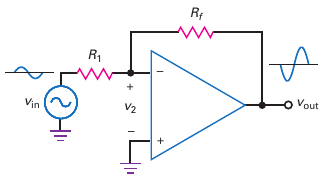
\includegraphics[height=0.5\textheight]{gambar/fig-16.12}
		\caption{Inverting amplifier}
		\label{fig-16.12}
	\end{figure}
\end{frame}

\subsection{Virtual Ground}
\begin{frame}{Virtual Ground}
	\begin{multicols}{2}
		\begin{figure}
			\centering
			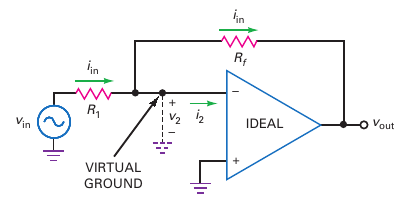
\includegraphics[height=0.4\textheight]{gambar/fig-16.13}
			\caption{Konsep virtual ground}
			\label{fig-16.13}
		\end{figure}
	\columnbreak
		\begin{itemize}
			\item Analisis inverting amplifier lebih mudah
			\item Berdasarkan op amp ideal:
			\begin{itemize}
				\item $ R_{in} = \infty \rightarrow i_2 = 0$
				\item $ A_{VOL} = \infty \rightarrow v_2 = 0 \rightarrow $
			\end{itemize}
			\item Karena $ i_2 = 0 $ maka $ i_{R_f} = i_{in} $
		\end{itemize}
	\end{multicols}
\end{frame}

\subsection{Voltage Gain \& Impedansi Input}
\begin{frame}{Voltage Gain \& Impedansi Input}
	\begin{multicols}{2}
		\begin{figure}
			\centering
			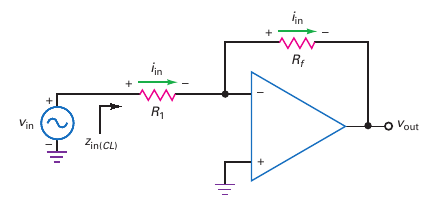
\includegraphics[height=0.4\textheight]{gambar/fig-16.14}
			\caption{Inverting amplifier memiliki arus yang sama yang melewati kedua resistor}
			\label{fig-16.14}
		\end{figure}
	\columnbreak
		\begin{itemize}
			\item Tegangan input: $ v_{in} = i_{in} R_1 $
			\item Tegangan output: $ v_{out} = -i_{in} R_f $
			\item Penguatan tegangan closed-loop:
			\begin{equation}\label{pers.16.3}
				A_{v(CL)} = \frac{-R_f}{R_1}
			\end{equation}
			%\item $ A_{v(CL)} < A_{VOL} $
			\item Impedansi input:
			\begin{equation}\label{pers.16.4}
				z_{in(CL)} = R_1
			\end{equation}
		\end{itemize}
	\end{multicols}
\end{frame}

\subsection{Bandwidth}
\begin{frame}{Bandwidth}
	\begin{multicols}{2}
		\begin{figure}
			\centering
			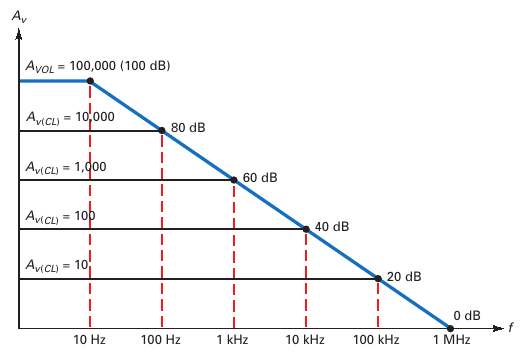
\includegraphics[height=0.6\textheight]{gambar/fig-16.15}
			\caption{Voltage gain yang lebih kecil menghasilkan bandwidth yang lebih besar}
			\label{fig-16.15}
		\end{figure}
	\columnbreak
		\begin{itemize}
			\item Closed-loop bandwidth:
			\begin{equation}\label{pers.16.5}
				f_{2(CL)} = \frac{f_{unity}}{dA_{v(CL)}}
			\end{equation}
			\item Gain-band-width product (GBW):
			\begin{equation}\label{pers.16.6}
				f_{unity} = A_{v(CL)}f_{2(CL)}
			\end{equation}
		\end{itemize}
	\end{multicols}
\end{frame}

\subsection{Bias dan Offset}
\begin{frame}{Bias dan Offset}
	content...
\end{frame}